フリーのMercedes F1 W14モデル
\footnote{
    実際のFormula 1には全部で10チーム20台のマシンが参加しておりそれぞれ異なるが,
    大まかな形状は同じである.
}
を使用して,$u=\SI{100}{\kilo\meter\per\hour}$とし,
実験をした結果の一部を以下\ref{fig:result-f1}に示す.
\footnote{
    実験の動画は以下のリンクから視聴できる.
    \url{https://youtu.be/rhfD4j8yjgk}
    \url{https://youtu.be/dGVB6DQThHI}
}
\footnote{
    FluidX3Dのバグとして,突然流体の速度が無限大に発散してしまうものが報告されている.
    \url{https://github.com/ProjectPhysX/FluidX3D/issues/109}.

    実際,次の動画のように,この実験でも突然流体の速度が無限大に発散してしまうことがあった.
    \url{https://youtu.be/PRkXo401tNI}.
    そのため本実験では,抗力・揚力の計算は行うことができなかった.

}



\begin{figure}[htbp]
    \begin{tabular}{cc}
        \begin{minipage}[b]{0.45\linewidth}
            \centering
            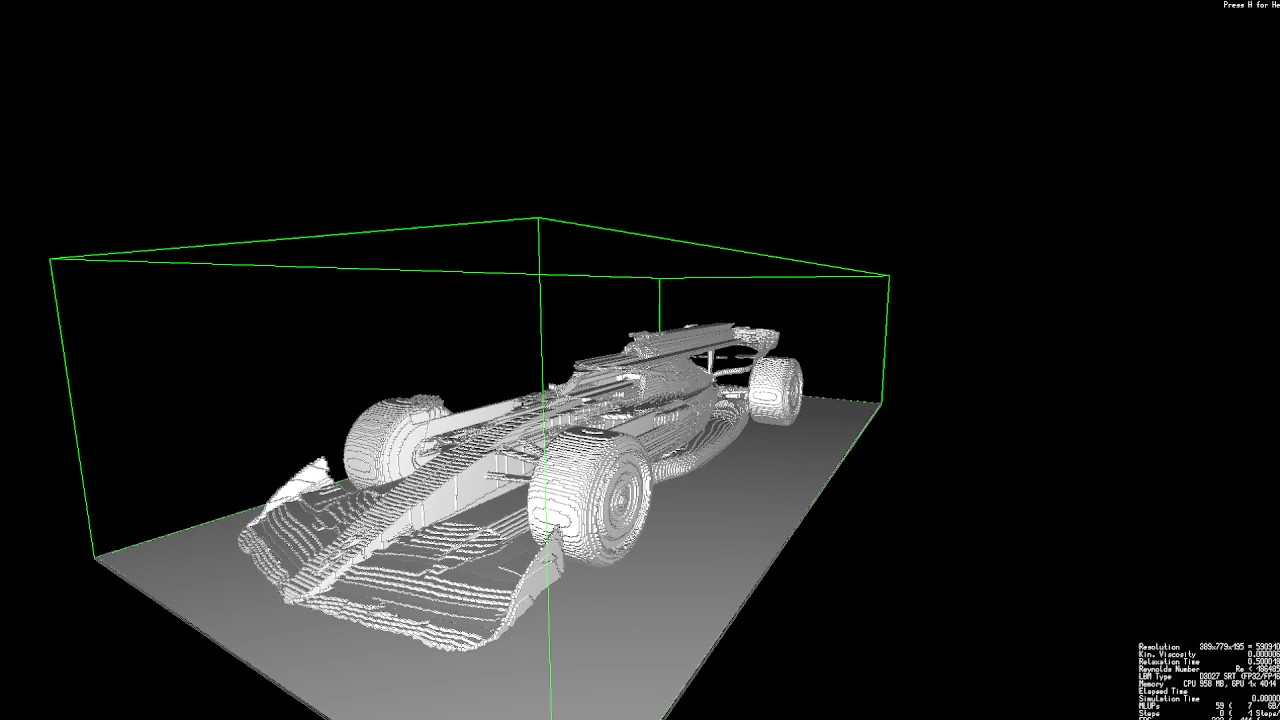
\includegraphics[width=0.9\linewidth]{figures/f1/2023-11-05 13-13-52 - frame at 0m0s.jpg}
            \subcaption{\SI{0}{\second}}
        \end{minipage}  &
        \begin{minipage}[b]{0.45\linewidth}
            \centering
            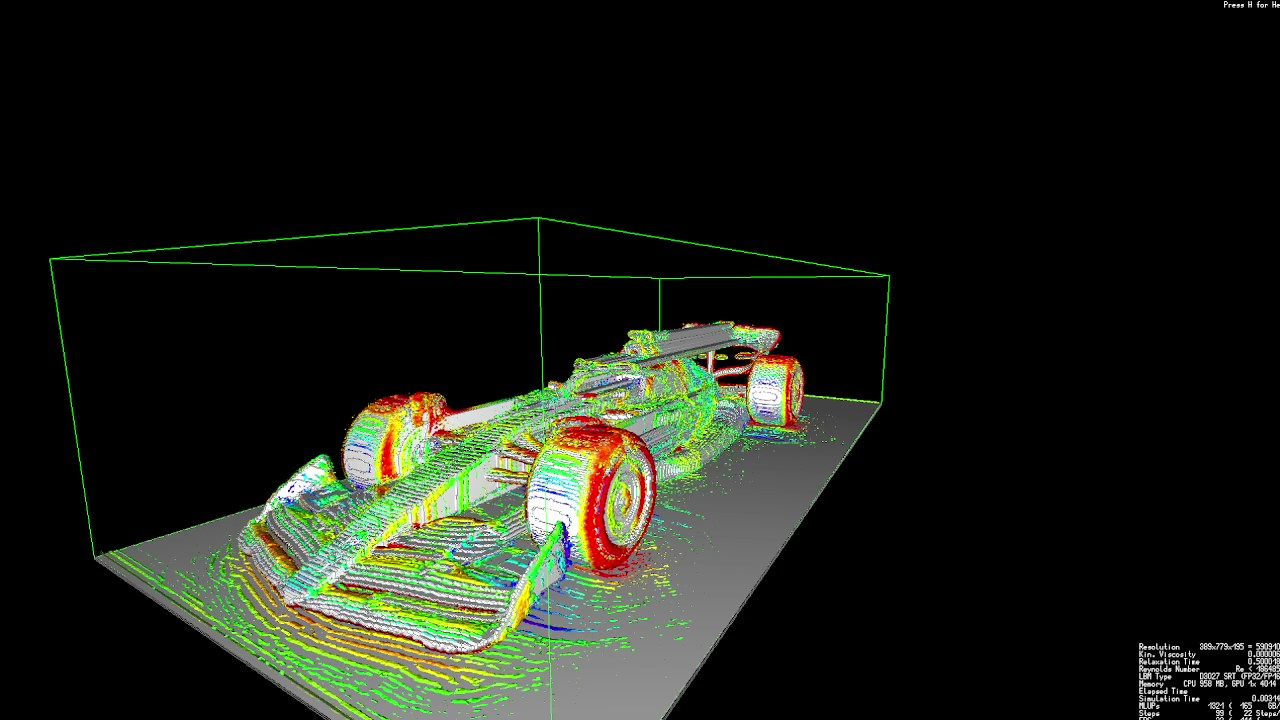
\includegraphics[width=0.9\linewidth]{figures/f1/2023-11-05 13-13-52 - frame at 0m7s.jpg}
            \subcaption{\SI{7}{\second}}
        \end{minipage}  \\
        \begin{minipage}[b]{0.45\linewidth}
            \centering
            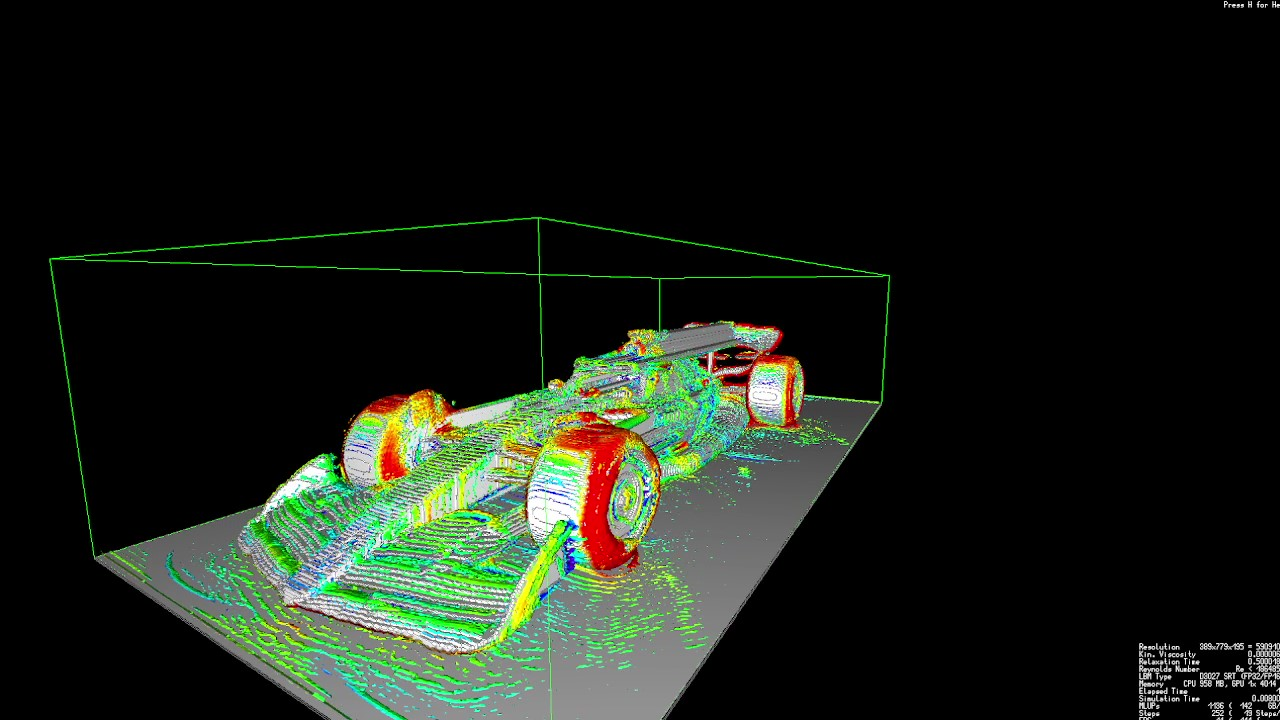
\includegraphics[width=0.9\linewidth]{figures/f1/2023-11-05 13-13-52 - frame at 0m14s.jpg}
            \subcaption{\SI{14}{\second}}
        \end{minipage} &
        \begin{minipage}[b]{0.45\linewidth}
            \centering
            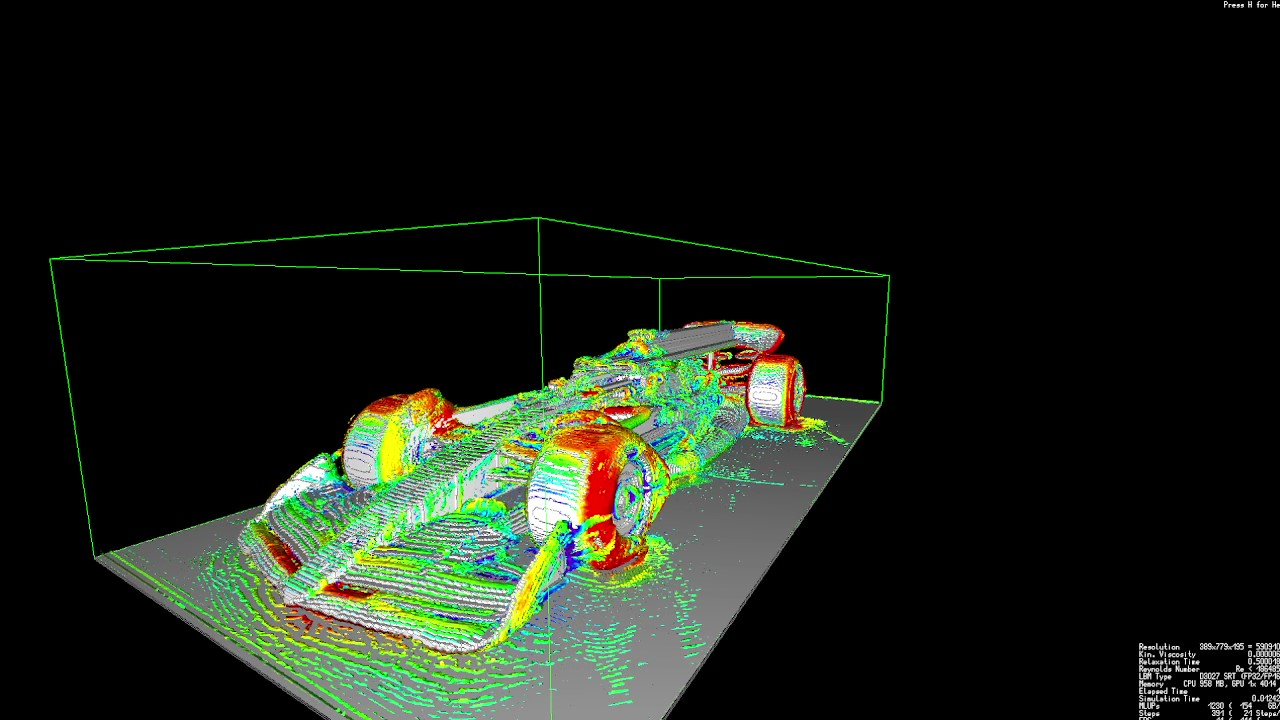
\includegraphics[width=0.9\linewidth]{figures/f1/2023-11-05 13-13-52 - frame at 0m21s.jpg}
            \subcaption{\SI{21}{\second}}
        \end{minipage} \\
        \begin{minipage}[b]{0.45\linewidth}
            \centering
            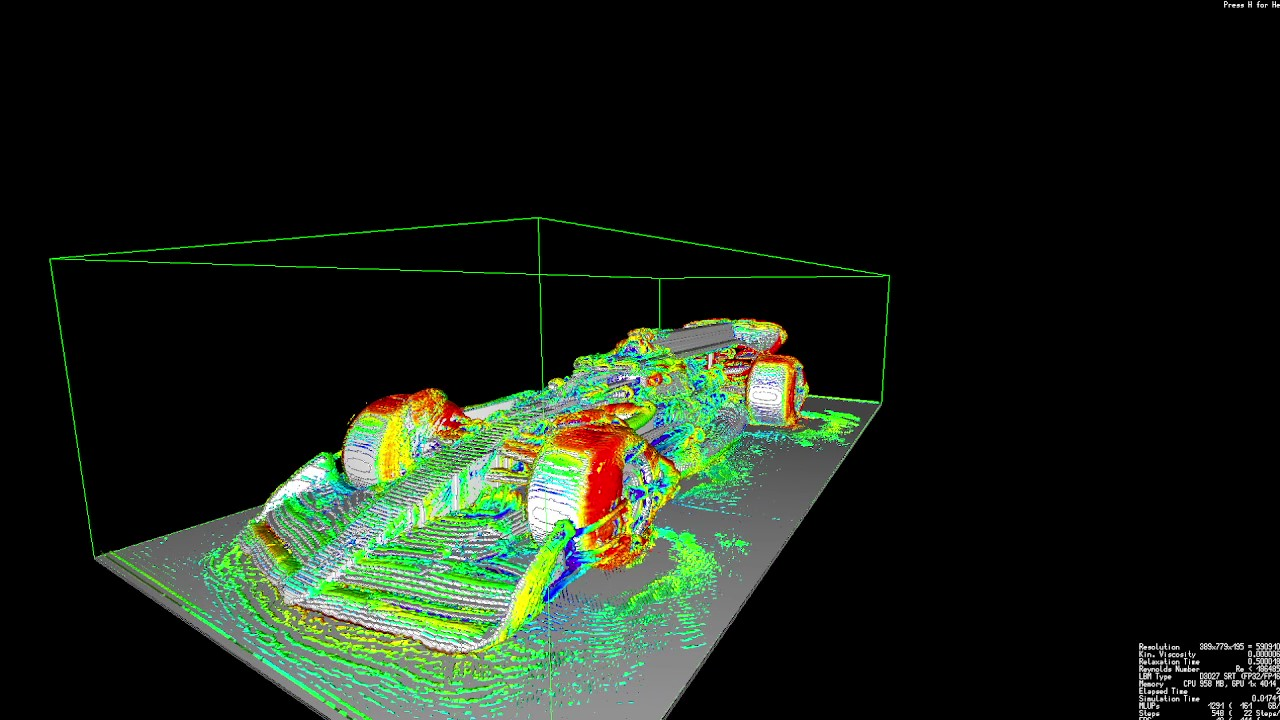
\includegraphics[width=0.9\linewidth]{figures/f1/2023-11-05 13-13-52 - frame at 0m28s.jpg}
            \subcaption{\SI{28}{\second}}
        \end{minipage} &
        \begin{minipage}[b]{0.45\linewidth}
            \centering
            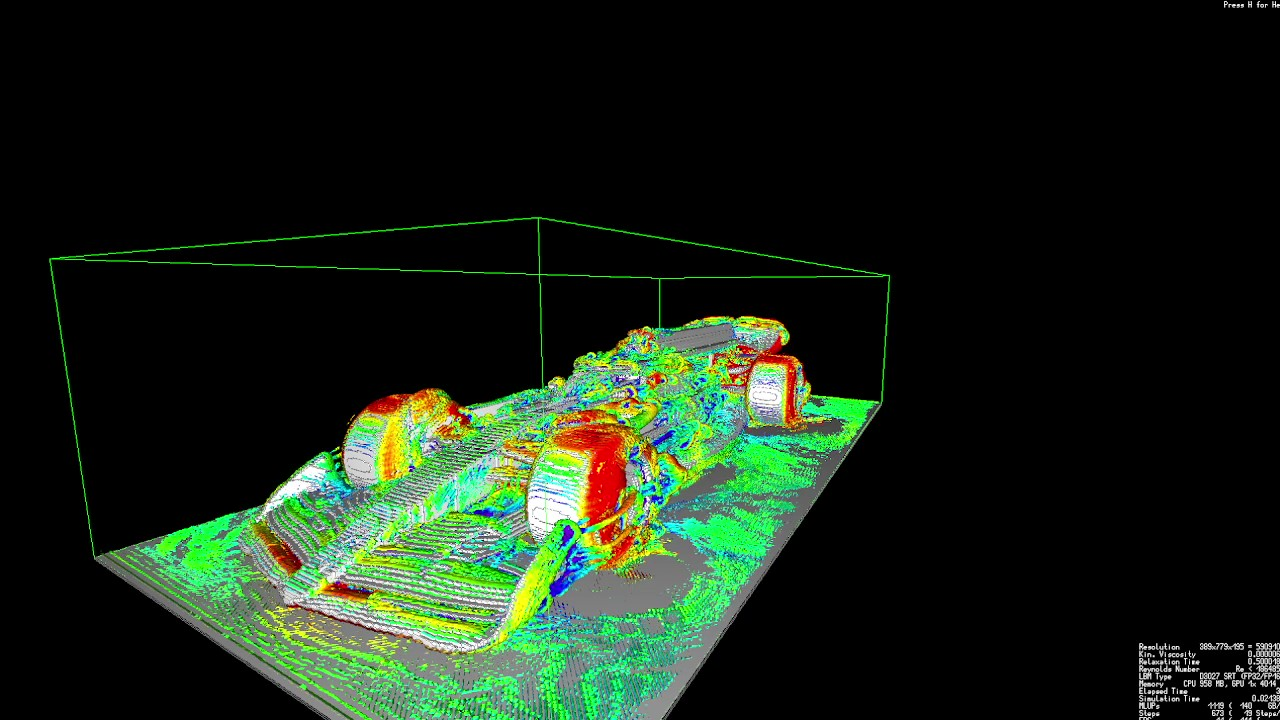
\includegraphics[width=0.9\linewidth]{figures/f1/2023-11-05 13-13-52 - frame at 0m35s.jpg}
            \subcaption{\SI{35}{\second}}
        \end{minipage} \\
        \begin{minipage}[b]{0.45\linewidth}
            \centering
            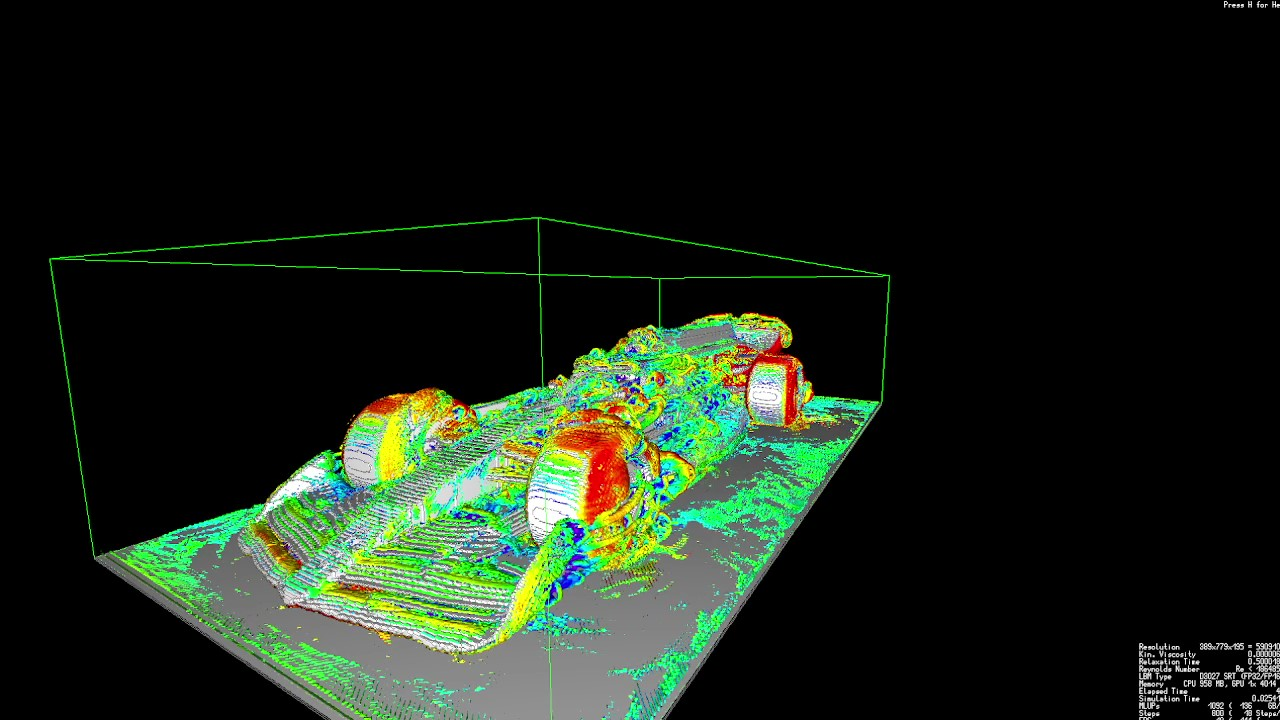
\includegraphics[width=0.9\linewidth]{figures/f1/2023-11-05 13-13-52 - frame at 0m42s.jpg}
            \subcaption{\SI{42}{\second}}
        \end{minipage} &
        \begin{minipage}[b]{0.45\linewidth}
            \centering
            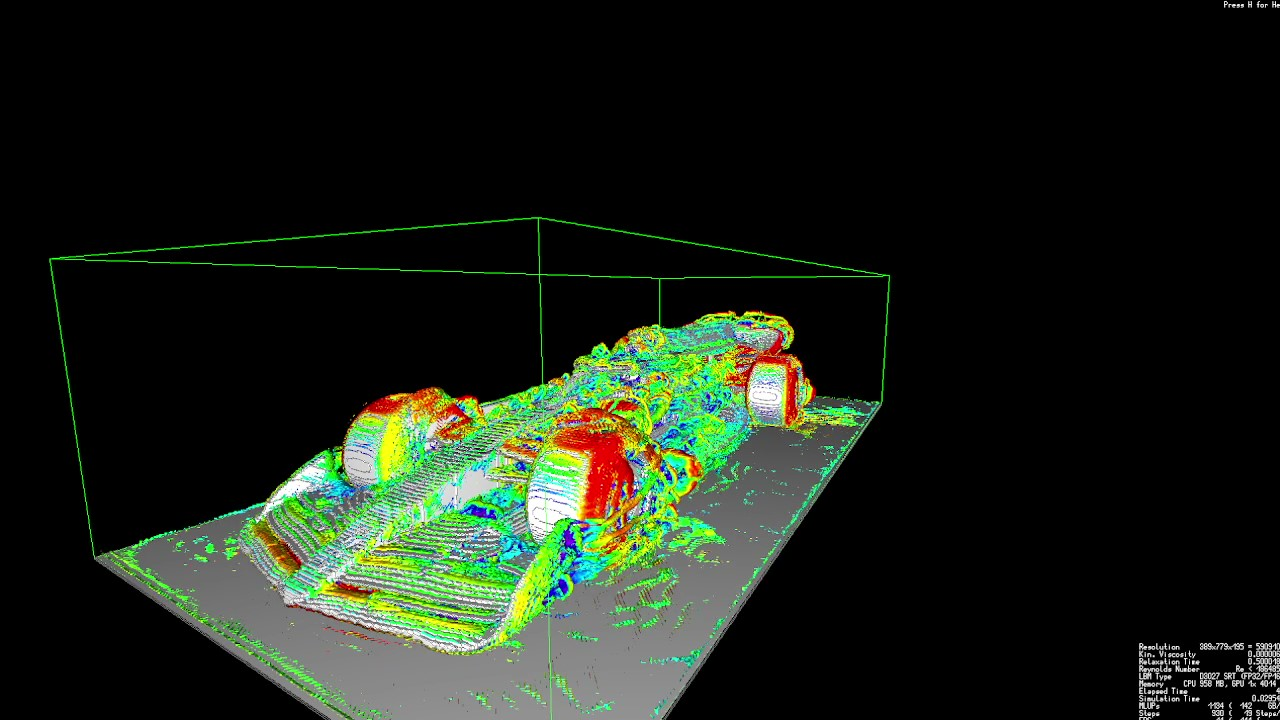
\includegraphics[width=0.9\linewidth]{figures/f1/2023-11-05 13-13-52 - frame at 0m49s.jpg}
            \subcaption{\SI{49}{\second}}
        \end{minipage} \\
        \begin{minipage}[b]{0.45\linewidth}
            \centering
            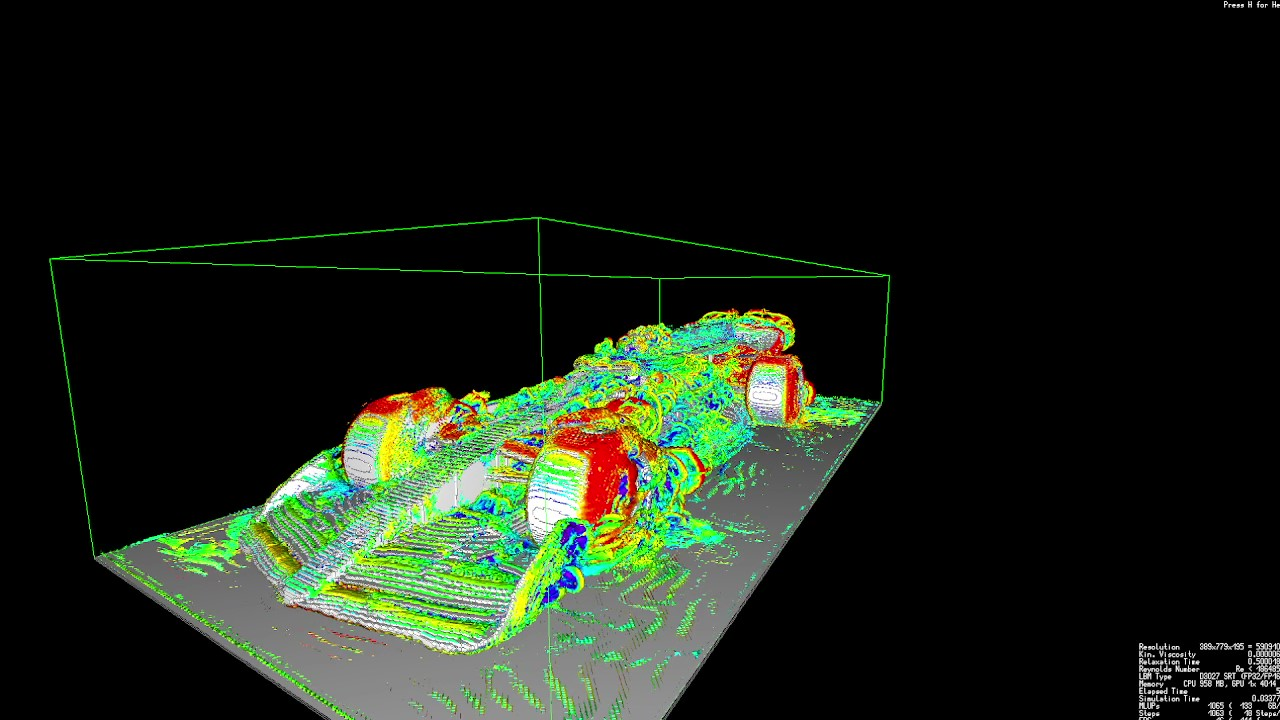
\includegraphics[width=0.9\linewidth]{figures/f1/2023-11-05 13-13-52 - frame at 0m56s.jpg}
            \subcaption{\SI{56}{\second}}
        \end{minipage} &
        \begin{minipage}[b]{0.45\linewidth}
            \centering
            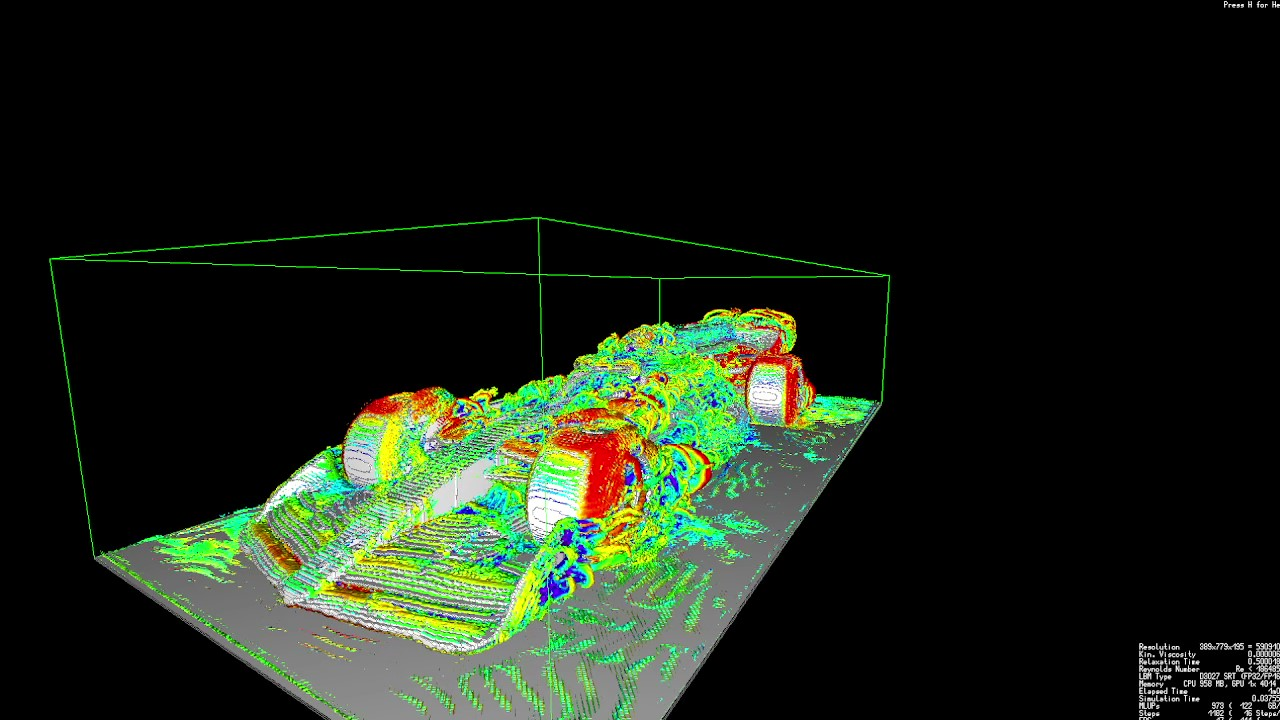
\includegraphics[width=0.9\linewidth]{figures/f1/2023-11-05 13-13-52 - frame at 1m3s.jpg}
            \subcaption{\SI{63}{\second}}
        \end{minipage}
    \end{tabular}

    \caption{Formula1 Mercedes W14の周りの空気の流れ}
    \label{fig:result-f1}
\end{figure}
